
\documentclass[twocolumn]{article}
\usepackage{mathpazo}
\usepackage{microtype}
\usepackage{times}

 %%%%%%%%%%%%%%%%%%%%%%%%%%%%%%%%%%%%%%%%%%%%%%%%%%%%%%%%%%%%%%%%%%%%%%%%%%%%%
 %                              My Commands
\newcommand{\bi}{\begin{itemize}}
\newcommand{\ei}{\end{itemize}}
\newcommand{\be}{\begin{enumerate}}
\newcommand{\ee}{\end{enumerate}}
\newcommand{\ii}{\item}
\newtheorem{Def}{Definition}
\newtheorem{Lem}{Lemma}
\usepackage{algorithm}
\usepackage{algorithmicx}
\usepackage{algpseudocode}
\usepackage{hhline}
%\usepackage{multirow}
%\usepackage{multicol}
\usepackage{graphicx}
\graphicspath{%
        {converted_graphics/}
        {./images/}
}
    
\setlength\textwidth{7in} 
\setlength\textheight{9.5in} 
\setlength\oddsidemargin{-0.25in} 
\setlength\topmargin{-0.25in} 
\setlength\headheight{0in} 
\setlength\headsep{0in} 
\setlength\columnsep{18pt}
\sloppy 
 
\begin{document}

\title{
\vspace{-0.5in}\rule{\textwidth}{2pt}
\begin{tabular}{ll}\begin{minipage}{4.75in}\vspace{6px}
\noindent\large Autonomous Control Middleware Research Section\\
\vspace{-12px}\\
\noindent\LARGE ETRI\qquad \large Technical Report 13VC1310-TR-05
\end{minipage}&\begin{minipage}{2in}\vspace{6px}\small
218 Gajeong-ro, Yuseong-gu\\
Daejeon, 305-700, South Korea\\
http:/$\!$/www.etri.re.kr/\quad 
\end{minipage}\end{tabular}
\rule{\textwidth}{2pt}\vspace{0.25in}
\LARGE \bf
Parallelism and Scientific Discovery
}

%\date{Autonomous Control Middleware Research Section, ETRI}

\author{
{\bf Sung-Soo Kim}\\
\it{sungsoo@etri.re.kr}
}

\maketitle

\begin{abstract}
This technical report describes the \emph{parallelism} in current computing environments related to \emph{scientific discovery, big data and analytics}.
In the past half century, parallel computers, parallel computation,
and scientific research have grown up together. Scientists
and researchers’ insatiable need to perform more and larger
computations has long exceeded the capabilities of conventional
computers. The only approach that has met this need is
parallelism -- computing more than one operation simultaneously.
At one level, parallelism is simple and easy to put into practice.
Building a parallel computer by replicating key operating components
such as the arithmetic units or even complete processors is
not difficult. But it is far more challenging to build a well-balanced
machine that is not stymied by internal bottlenecks. In the end,
the principal problem has been software, not hardware. Parallel
programs are far more \emph{difficult} to design, write, debug, and tune
than sequential software -- which itself is still not a mature, reproducible
artifact.

\end{abstract}

\section{Introduction}
\subsection{The Evolution of Parallel Computing}
The evolution of successive generations of parallel computing
hardware has also forced a \emph{constant rethinking} of parallel algorithms
and software. Early machines such as the IBM Stretch, the
Cray I, and the Control Data Cyber series all exposed parallelism
as vector operations. The Cray II, Encore, Alliant, and many generations
of IBM machines were built with multiple processors that
shared memory. Because it proved so difficult to increase the number of processors
while sharing a single memory, designs evolved further into systems in which
no memory was shared and processors shared information by passing messages.
Beowulf clusters, consisting of racks of standard PCs connected by Ethernet,
emerged as an economical approach to supercomputing. Networks improved in
latency and bandwidth, and this form of distributed computing now dominates supercomputers.
Other systems, such as the Cray multi-threaded platforms, demonstrated
that there were different approaches to addressing shared-memory parallelism.
While the scientific computing community has struggled with programming
each generation of these exotic machines, the mainstream computing world has
been totally satisfied with sequential programming on machines where any parallelism
is hidden from the programmer deep in the hardware.

In the past few years, parallel computers have entered mainstream computing
with the advent of multicore computers. Previously, most computers were sequential
and performed a single operation per time step. Moore’s Law drove the improvements
in semiconductor technology that doubled the transistors on a chip
every two years, which increased the clock speed of computers at a similar rate
and also allowed for more sophisticated computer implementations. As a result,
computer performance grew at roughly 40\% per year from the 1970s, a rate that
satisfied most software developers and computer users. This steady improvement
ended because increased clock speeds require more power, and at approximately
3 GHz, chips reached the limit of economical cooling. Computer chip manufacturers,
such as Intel, AMD, IBM, and Sun, shifted to multicore processors that used
each Moore’s Law generation of transistors to double the number of independent
processors on a chip. Each processor ran no faster than its predecessor, and sometimes
even slightly slower, but in aggregate, a multicore processor could perform
twice the amount of computation as its predecessor.

\subsection{Parallel Programming Challenges}
This new computer generation rests on the same problematic foundation of software
that the scientific community struggled with in its long experience with parallel
computers. Most existing general-purpose software is written for sequential
computers and will not run any faster on a multicore computer. Exploiting the potential
of these machines requires new, parallel software that can break a task into
multiple pieces, solve them more or less independently, and assemble the results
into a single answer. Finding better ways to produce parallel software is currently
the most pressing problem facing the software development community and is the
subject of considerable research and development.
The scientific and engineering communities can both benefit from these urgent
efforts and can help inform them. Many parallel programming techniques originated
in the scientific community, whose experience has influenced the search for
new approaches to programming multicore computers. Future improvements in
our ability to program multicore computers will benefit all software developers as
the distinction between the leading-edge scientific community and general-purpose
computing is erased by the inevitability of parallel computing as the fundamental
programming paradigm.

One key problem in parallel programming today is that most of it is conducted
at a very \emph{low level of abstraction}. Programmers must break their code into components
that run on specific processors and communicate by writing into shared
memory locations or exchanging messages. In many ways, this state of affairs is
similar to the early days of computing, when programs were written in assembly
languages for a specific computer and had to be rewritten to run on a different
machine. In both situations, the problem was not just the lack of reusability of programs,
but also that assembly language development was less productive and more
error prone than writing programs in \emph{higher-level languages}.

\subsection{Addressing the Challenges}
Several lines of research are attempting to raise the level at which parallel programs
can be written. The oldest and best-established idea is data parallel programming.
In this programming paradigm, an operation or sequence of operations is applied
simultaneously to all items in a collection of data. The granularity of the operation
can range from adding two numbers in a data parallel addition of two matrices
to complex data mining calculations in a \emph{map-reduce style} computation. The
appeal of data parallel computation is that parallelism is mostly hidden from the
programmer. Each computation proceeds in isolation from the concurrent computations
on other data, and the code specifying the computation is sequential. The
developer need not worry about the details of moving data and running computations
because they are the responsibility of the runtime system. GPUs (graphics
processing units) provide hardware support for this style of programming, and they
have recently been extended into GPGPUs(general-purpose GPUs) that perform
very high-performance numeric computations.

Unfortunately, \emph{data parallelism} is not a programming model that works for all
types of problems. Some computations require more communication and coordination.
For example, \emph{protein folding} calculates the forces on all atoms in parallel, but
local interactions are computed in a manner different from remote interactions.
Other examples of computations that are hard to write as data parallel programs
include various forms of \emph{adaptive mesh refinement} that are used in many modern
physics simulations in which local structures, such as clumps of matter or cracks in
a material structure, need finer spatial resolution than the rest of the system.

A new idea that has recently attracted considerable research attention is \emph{transactional
memory} (TM), a mechanism for coordinating the sharing of data in a
multicore computer. \emph{Data sharing} is a rich source of programming errors because
the developer needs to ensure that a processor that changes the value of data has
exclusive access to it. If another processor also tries to access the data, one of the
two updates can be lost, and if a processor reads the data too early, it might see an
inconsistent value. The most common mechanism for preventing this type of error
is a lock, which a program uses to prevent more than one processor from accessing
a memory location simultaneously. Locks, unfortunately, are low-level mechanisms
that are easily and frequently misused in ways that both allow concurrent access
and cause deadlocks that freeze program execution.

TM is a \emph{higher-level abstraction} that allows the developer to identify a group of
program statements that should execute \emph{atomically} -- that is, as if no other part of
the program is executing at the same time. So instead of having to acquire locks for
all the data that the statements might access, the developer shifts the burden to the
runtime system and hardware. TM is a promising idea, but many engineering challenges
still stand in the way of its widespread use. Currently, TM is expensive to implement
without support in the processors, and its usability and utility in large, real-world
codes is as yet undemonstrated. If these issues can be resolved, TM promises
to make many aspects of multicore programming far easier and less error prone.

Another new idea is the use of \emph{functional programming languages}. These languages
embody a \emph{style of programming} that mostly \emph{prohibits updates to program
state}. In other words, in these languages a variable can be given an initial value,
but that value cannot be changed. Instead, a new variable is created with the new
value. This style of programming is well suited to parallel programming because
it eliminates the updates that require synchronization between two processors.
Parallel, functional programs generally use \emph{mutable state} only for communication
among parallel processors, and they require locks or TM only for this small, distinct
part of their data.

Until recently, only the scientific and engineering communities have struggled
with the difficulty of using parallel computers for anything other than the most
embarrassingly parallel tasks. The advent of \emph{multicore processors} has changed this
situation and has turned parallel programming into a major challenge for all software
developers. The new ideas and programming tools developed for mainstream
programs will likely also benefit the technical community and provide it with new
means to take better advantage of the continually increasing power of multicore
processors.

\section{Parallelism and the Cloud}
Cloud and cloud technologies are two broad categories of technologies related to the general notion of \emph{Cloud Computing}. 
By  {\bfseries Cloud}, we refer to a collection of infrastructure services such as \emph{Infrastructure-as-a-service} (IaaS), \emph{Platform-as-a-Service} (PaaS), etc., provided by various organizations where virtualization plays a key role. 
By  {\bfseries Cloud Technologies}, we refer to various cloud runtimes such as Hadoop, Dryad, and other MapReduce frameworks, and also the storage and communication frameworks such as \emph{Hadoop Distributed File System} (HDFS), Amazon S3, etc.

Figure \ref{HDFSOverview} shows the overview of HDFS architecture.
In HDFS, the daemon responsible for storing and retrieving block data is called the \emph{datanode} (DN). The datanode has direct local access to one or more disks—commonly called data disks —in a server on which it’s permitted to store block data. In production systems, these disks are usually reserved exclusively for Hadoop. Storage can be added to a cluster by adding more datanodes with additional disk capacity, or even adding disks to existing datanodes.

One of the most striking aspects of HDFS is that it is designed in such a way that it doesn’t require RAID storage for its block data. This keeps with the commodity hard- ware design goal and reduces cost as clusters grow in size. Rather than rely on a RAID controller for data safety, block data is simply written to multiple machines. This fulfills the safety concern at the cost of raw storage consumed; however, there’s a performance aspect to this as well. Having multiple copies of each block on separate machines means that not only are we protected against data loss if a machine disappears, but during processing, any copy of this data can be used. By having more than one option, the scheduler that decides where to perform processing has a better chance of being able
to find a machine with available compute resources and a copy of the data.
\begin{figure}[htb]
	\centering
	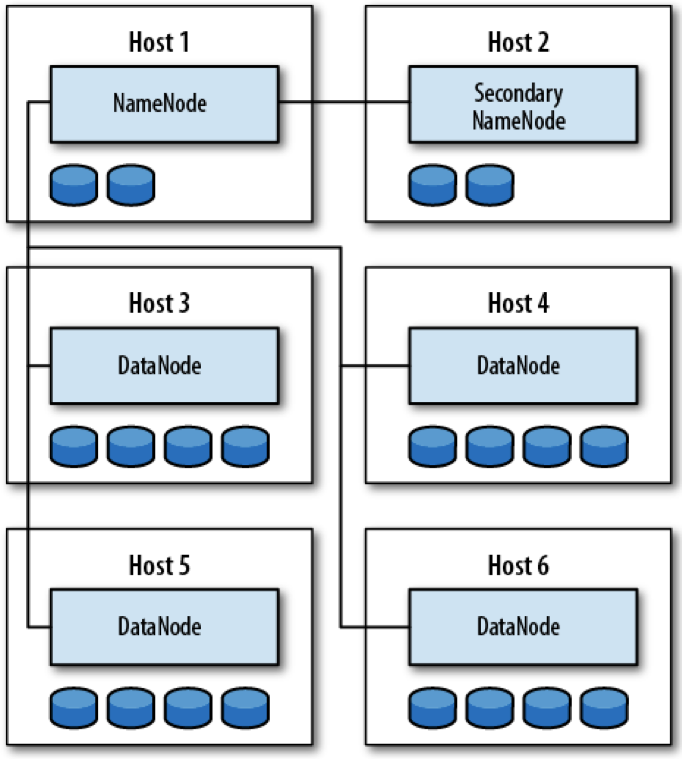
\includegraphics[width=0.4\textwidth]{HDFSOverview}
	\caption{HDFS architecture overview}
	\label{HDFSOverview}
\end{figure}

While datanodes are responsible for storing block data, the \emph{namenode} (NN) is the daemon that stores the filesystem metadata and maintains a complete picture of the filesystem. Clients connect to the namenode to perform filesystem operations; al- though, as we’ll see later, block data is streamed to and from datanodes directly, so bandwidth is not limited by a single node. Datanodes regularly report their status to the namenode in a heartbeat. This means that, at any given time, the namenode has a complete view of all datanodes in the cluster, their current health, and what blocks they have available. 

Over the past decade, scientific and engineering research via computing has emerged as the third pillar of the scientific process, complementing theory and experiment. Several national studies have highlighted the importance of computational science as a critical enabler of scientific discovery and national competitiveness in the physical and biological sciences, medicine and healthcare, and design and manufacturing \cite{NITRD:2005, Reed:2003, Graham:2004}. 

As the term suggests, computational science has historically focused on \emph{computation}: the creation and execution of mathematical models of natural and artificial processes. Driven by opportunity and necessity, computational science is expanding to encompass both \emph{computing} and \emph{data analysis}. Today, a rising tsunami of data threatens to overwhelm us, consuming our attention by its very volume and diversity. Driven by inexpensive, seemingly ubiquitous sensors, broadband networks, and high-capacity storage systems, the tsunami encompasses data from sensors that monitor our planet from deep in the ocean, from land instruments, and from space-based imaging systems. It also includes environmental measurements and healthcare data that quantify biological processes and the effects of surrounding conditions. Simply put, we are moving from \emph{data paucity} to a \emph{data plethora}, which is leading to a relative poverty of human attention to any individual datum and is necessitating machine-assisted winnowing.

This ready availability of diverse data is shifting scientific approaches from the
traditional, \emph{hypothesis-driven scientific method} to science based on exploration. Researchers no longer simply ask, "What experiment could I construct to test this hypothesis?" Increasingly, they ask, "What correlations can I glean from extant data?" More tellingly, one wishes to ask, \emph{"What insights could I glean if I could fuse data from multiple disciplines and domains?"}. 
 The challenge is analyzing many petabytes of data on a time scale that is practical in human terms.
Figure \ref{Analytics} shows the typical concept of the agile analytics process in common business environments.
\begin{figure}[htb]
	\centering
	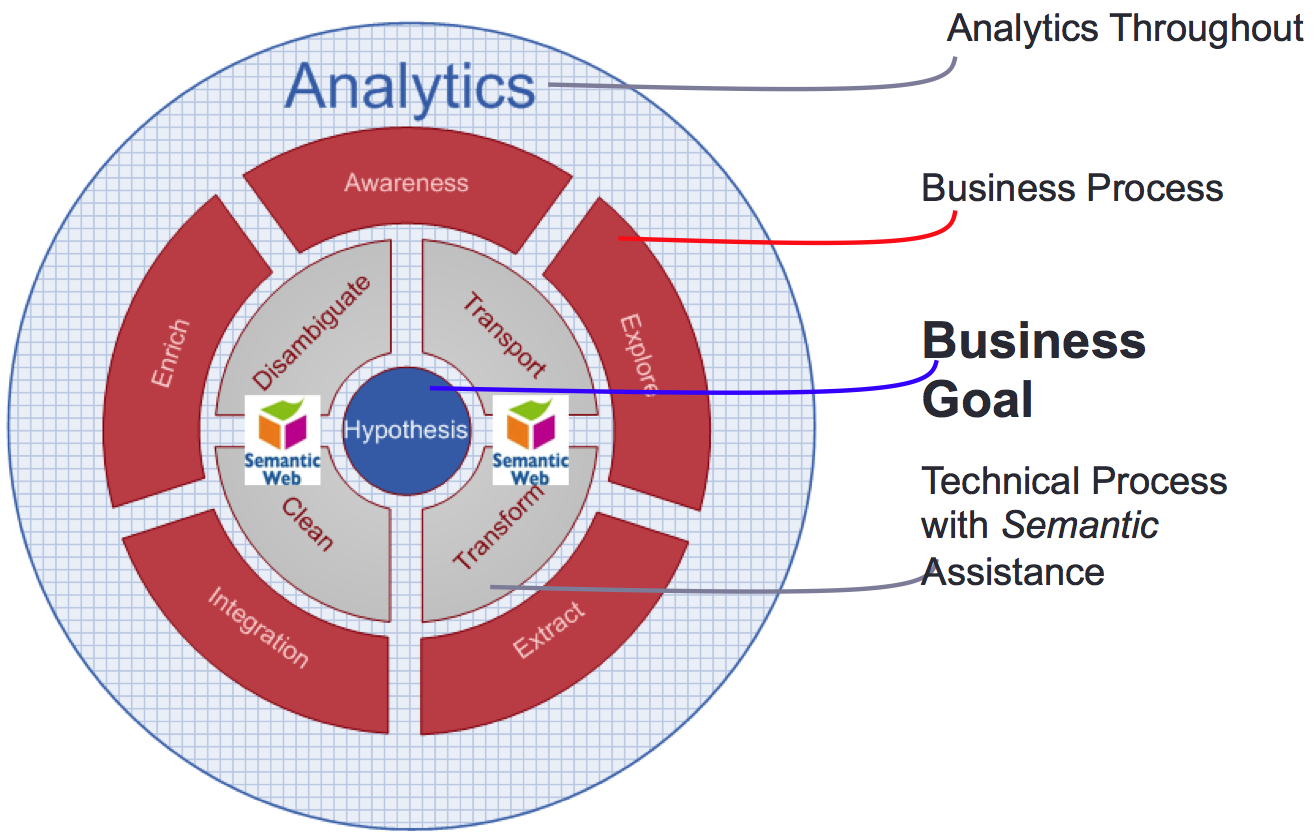
\includegraphics[width=0.48\textwidth]{AnalyticProcess}
	\caption{Agile Anaytics Process}
	\label{Analytics}
\end{figure}

The ability to create rich, detailed models of natural and artificial phenomena and to process large volumes of experimental data created by a new generation of scientific instruments that are themselves powered by computing makes computing a \emph{universal intellectual amplifier}, advancing all of science and engineering and powering the knowledge economy. Cloud computing is the latest technological evolution of computational science, allowing groups to host, process, and analyze large volumes of multidisciplinary data. Consolidating computing and storage in very large datacenters creates economies of scale in facility design and construction, equipment acquisition, and operations and maintenance that are not possible when these elements are distributed. Moreover, consolidation and hosting mitigate many of the sociological and technical barriers that have limited multidisciplinary data sharing and collaboration. Finally, cloud hosting facilitates long-term data preservation—a task that is particularly challenging for universities and government agencies and is critical to our ability to conduct longitudinal experiments. 

It is not unreasonable to say that modern datacenters and modern supercomputers are like twins separated at birth. Both are massively parallel in design, and both are organized as a network of communicating computational nodes. The individual nodes of each are based on commodity microprocessors that have multiple cores, large memories, and local disk storage. They both execute applications that are designed to exploit massive amounts of parallelism. Their differences lie in their evolution. Massively parallel supercomputers have been designed to support computation with occasional bursts of input/output and to complete a single massive calculation as fast as possible, one job at a time. In contrast, datacenters direct their power outward to the world and consume vast quantities of input data.

Parallelism can be exploited in cloud computing in two ways. The first is for \emph{human access}. Cloud applications are designed to be accessed as Web services, so they are organized as two or more layers of processes. One layer provides the service interface to the user’s browser or client application. This {\bfseries Web role} layer accepts users’ requests and manages the tasks assigned to the second layer. The second layer of processes, sometimes known as the {\bfseries worker role} layer, executes the analytical tasks required to satisfy user requests. One Web role and one worker role may be sufficient for a few simultaneous users, but if a cloud application is to be widely used -- such as for search, customized maps, social networks, weather services, travel data, or online auctions—it must support thousands of concurrent users.

The second way in which \emph{parallelism} is exploited involves the nature of the \emph{data analysis} tasks undertaken by the application. In many large data analysis scenarios, it is not practical to use a single processor or task to scan a massive dataset or data stream to look for a pattern -- the overhead and delay are too great. In these cases, one can partition the data across large numbers of processors, each of which can analyze a subset of the data. The results of each {\bfseries sub-scan} are then combined and returned to the user.

This \emph{map-reduce pattern} is frequently used in datacenter applications and is one in a broad family of parallel data analysis queries used in cloud computing. 
Web search is the canonical example of this \emph{two-phase model}. It involves constructing a searchable keyword index of the Web's contents, which entails creating a copy of the Web and sorting the contents via a sequence of map-reduce steps. 
{\bfseries Three key technologies} support this model of parallelism: Google has an internal version \cite{Dean:2004}, Yahoo! has an open source version known as \emph{Hadoop}, and Microsoft has a map- reduce tool known as DryadLINQ \cite{Isard:2008}. 

Dryad is a mechanism to support the execution of distributed collections of tasks that can be configured into an arbitrary \emph{directed acyclic graph} (DAG). 
The \emph{Language Integrated Query} (LINQ) extension to C$\#$ allows SQL-like query expressions to be embedded directly in regular programs. 
The goal of DryadLINQ is to make distributed computing on large compute cluster simple enough for every programmer. DryadLINQ combines two important pieces of Microsoft technology: the \emph{Dryad distributed execution engine} and the .NET \emph{Language Integrated Query} (LINQ).
Figure \ref{dryad} shows the typical process of the DryadLINQ.
The DryadLINQ system can automatically compile these queries into Dryad DAG, which can be executed automatically in the cloud.
\begin{figure}[htb]
	\centering
	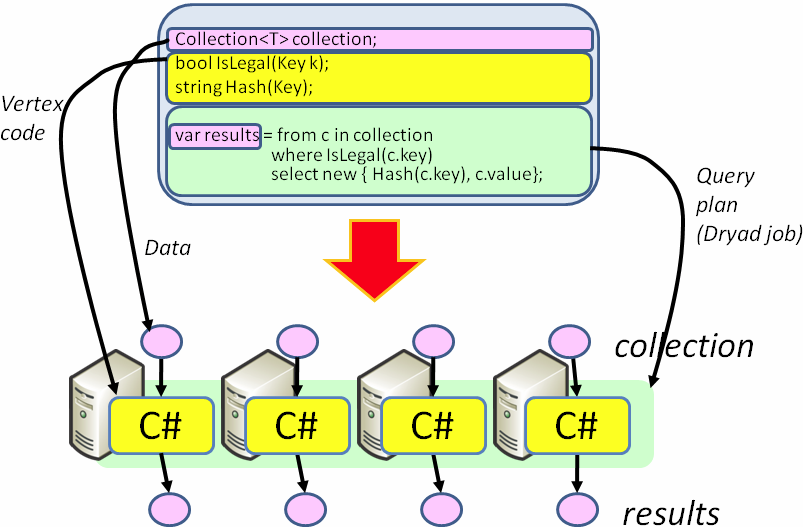
\includegraphics[width=0.45\textwidth]{dryad}
	\caption{DryadLINQ Process}
	\label{dryad}
\end{figure}

DryadLINQ translates LINQ programs into distributed Dryad computations:
\begin{itemize}
  \item C\# and LINQ data objects become distributed partitioned files.
  \item LINQ queries become distributed Dryad jobs.
  \item C\# methods become code running on the vertices of a Dryad job.
\end{itemize}

DryadLINQ has the following features:
\begin{itemize}
  \item {\bfseries Declarative programming:} computations are expressed in a high-level language containing a superset of the best features of SQL, functional programming and .Net.
  \item {\bfseries Automatic parallelization:} from sequential declarative code the DryadLINQ compiler generates highly parallel query plans spanning large computer clusters. DryadLINQ also exploits multi-core parallelism on each machine.
  \item {\bfseries Integration with Visual Studio:} programmers in DryadLINQ take advantage of the comprehensive VS set of tools: Intellisense, code refactoring, integrated debugging, build, source code management.
  \item {\bfseries Integration with .Net:} all .Net libraries, including Visual Basic, and dynamic languages are available.
  \item {\bfseries Type safety:} distributed computations are statically type-checked.
  \item {\bfseries Automatic serialization:} data transport mechanisms automatically handle all .Net object types.
  \item {\bfseries Job graph optimizations}
	\begin{itemize}
		\item \emph{static}: a rich set of term-rewriting query optimization rules is applied to the query plan, optimizing locality and improving performance.
		\item \emph{dynamic}: run-time query plan optimizations automatically adapt the plan taking into account the statistics of the data set processed.
	\end{itemize}
  \item {\bfseries Conciseness:} the following line of code is a complete implementation of the Map-Reduce computation framework in DryadLINQ:
\end{itemize}

Microsoft Windows Azure supports a combination of multi-user scaling and data analysis parallelism. In Azure, applications are designed as stateless \emph{roles} that fetch tasks from queues, execute them, and place new tasks or data into other queues. Map-reduce computations in Azure consist of two pools of worker roles: mappers, which take map tasks off a map queue and push data to the Azure storage, and reducers, which look for reduce tasks that point to data in the storage system that need reducing. Whereas DryadLINQ executes a \emph{static} DAG, Azure can execute an \emph{implicit} DAG in which nodes correspond to roles and links correspond to messages in queues. Azure computations can also represent the parallelism generated by very large numbers of concurrent users.

This same type of map-reduce data analysis appears repeatedly in large-scale scientific analyses. For example, consider the task of matching a DNA sample against the thousands of known DNA sequences as shown in Figure \ref{DNA} . This kind of search is an \emph{embarrassingly parallel} task that can easily be sped up if it is partitioned into many independent search tasks over subsets of the data. Similarly, consider the task of searching for patterns in medical data, such as to find anomalies in fMRI scans of brain images, or the task of searching for potential weather anomalies in streams of events from radars.
\begin{figure}[htb]
	\centering
	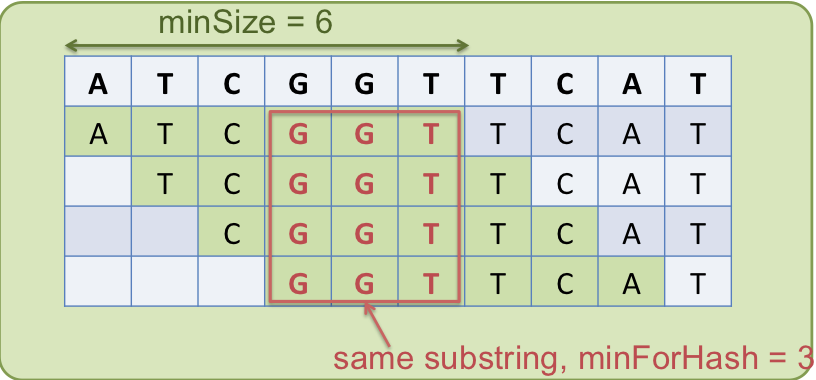
\includegraphics[width=0.4\textwidth]{matchingDNA}
	\caption{Matching DNA substrings}
	\label{DNA}
\end{figure}

Finally, another place where parallelism can be exploited in the datacenter is at the hardware level of an individual node. Not only does each node have multiple processors, but each typically has multiple computer cores. For many data analysis tasks, one can exploit massive amounts of parallelism at the instruction level. For example, filtering noise from sensor data may involve invoking a Fast Fourier Transform (FFT) or other spectral methods. These computations can be sped up by using general-purpose graphics processing units (GPGPUs) in each node. Depend- ing on the rate at which a node can access data, this GPGPU-based processing may allow us to decrease the number of nodes required to meet an overall service rate.

\section{Conclusion}
The World Wide Web began as a loose federation of simple Web servers that each hosted scientific documents and data of interest to a relatively small community of researchers. As the number of servers grew exponentially and the global Internet matured, Web search transformed what was initially a scientific experiment into a new economic and social force. The effectiveness of search was achievable only because of the available parallelism in massive datacenters. As we enter the period in which all of science is being driven by a data explosion, cloud computing and its inherent ability to exploit parallelism at many levels has become a fundamental new enabling technology to advance human knowledge.

\bibliographystyle{IEEEtran}
\bibliography{References}


\end{document}
